\documentclass[10pt,conference]{IEEEtran}
\IEEEoverridecommandlockouts
% The preceding line is only needed to identify funding in the first footnote. If that is unneeded, please comment it out.
\usepackage{cite}
\usepackage{amsmath,amssymb,amsfonts}
%\usepackage{algorithmic}
\usepackage{graphicx}
\usepackage{textcomp}
\usepackage{xcolor}
\usepackage{tikz}
\usepackage{multirow}
\usetikzlibrary{arrows.meta}
\usepackage{subcaption}
\usepackage{todonotes}
\usepackage{multirow}
\usepackage{xspace}
\usepackage{hyperref}
\usepackage{url}
\usepackage{comment}

\def\BibTeX{{\rm B\kern-.05em{\sc i\kern-.025em b}\kern-.08em
    T\kern-.1667em\lower.7ex\hbox{E}\kern-.125emX}}
\begin{document}

\newcommand\schim{SchIM\xspace}
\newcommand\schimL{Scheduler In-the-Middle\xspace}
\newcommand\schiml{scheduler in-the-middle\xspace}
\newcommand\axiin[1]{$\texttt{HPM}_{#1}$\xspace}
\newcommand\axiout[1]{$\texttt{HPS}_{#1}$\xspace}
\newcommand\axiconf[1]{$\texttt{LPM}_{#1}$\xspace}

\newcommand{\fig}[1]{Fig.~\ref{#1}}

\newcommand*\circledfig[2]{Fig.~\ref{#1}\tikz[baseline=0pt]{\node[anchor=south west,red,shape=circle,draw,inner sep=1pt] (char) {\scriptsize#2};}}

\newcommand*\circled[1]{\tikz[baseline=0pt]{\node[anchor=south west,red,shape=circle,draw,inner sep=1pt] (char) {\scriptsize#1};}}

\title{A Memory Scheduling Infrastructure for Multi-core Systems with
  Re-programmable Logic
%    \thanks{Identify applicable funding agency here. If none, delete this.}
}

\author{
%    \IEEEauthorblockN{1\textsuperscript{st} Given Name Surname}
%    \IEEEauthorblockA{
%        \textit{dept. name of organization (of Aff.)} \\
%        \textit{name of organization (of Aff.)}\\
%        City, Country \\
%        email address or ORCID
%    }
%    \and
%    \IEEEauthorblockN{2\textsuperscript{nd} Given Name Surname}
%    \IEEEauthorblockA{
%        \textit{dept. name of organization (of Aff.)} \\
%        \textit{name of organization (of Aff.)}\\
%        City, Country \\
%        email address or ORCID
%    }
%    \and
%    \IEEEauthorblockN{3\textsuperscript{rd} Given Name Surname}
%    \IEEEauthorblockA{
%        \textit{dept. name of organization (of Aff.)} \\
%        \textit{name of organization (of Aff.)}\\
%        City, Country \\
%        email address or ORCID
%    }
    Authors omitted for review.
}

\maketitle

\begin{abstract}


The sharp increase in demand for performance has prompted an explosion
in the complexity of modern multi-core embedded systems. This has lead
to unprecedented temporal unpredictability concerns in Cyber-Physical
Systems (CPS). On-chip integration of programmable logic (PL)
alongside a conventional Processing Systems (PS) in modern
Systems-on-Chip (SoC) establishes a genuine compromise between
specialization, performance, and re-configurability. In addition to
typical use-cases, it has been shown that the PL can be used to
observe, manipulate, and ultimately manage memory traffic generated by
a traditional multi-core processor.

This paper explores the possibility of PL-aided memory scheduling by
proposing a \schimL (\schim). We demonstrate that the \schim enables
transaction-level control over the main memory traffic generated by a
set of embedded cores. Focusing on extensibility and
reconfigurability, we put forward a \schim design covering two main
objectives. First, to provide a safe playground to test innovative
memory scheduling mechanisms; and second, to establish a transition
path from software-based memory regulation to provably correct
hardware-enforced memory scheduling. We evaluate our design through a
full-system implementation on a commercial PS-PL platform using
synthetic and real-world benchmarks.
\end{abstract}

\begin{IEEEkeywords}
component, formatting, style, styling, insert
\end{IEEEkeywords}

\section{Introduction}
    In modern embedded Mutli-core Systems, caches have become an angular piece of hardware bridging the gap between the speed of the connected execution units and the main memory. With the growing demand for high-performance multi-core system on chips, shared caches have evolved to accomodate the many concurrent accesses to main memory. These caches are referred to as \emph{non-blocking}.\\

    Unfortunately, while non-blocking shared caches offer great average perfomance, their behaviour is opaque and unpredictable. Dealing with the cache behaviour is of the utmost importance for safety critical hard Real-Time systems where timing constraints must be respected. A great deal of research has been conducted on cache management for Real-Time applications on MPSoCs. The two main sources of unpredictability imputed to the last level of cache are (1) the inter-core cache line eviction and (2) the opaque management of internaly shared resources.

    The inter-core cache line eviction is a well studied source of unpredictability that arises when the memory accesses of two independent cores lead to the eviction of each others cache line in a destructive way. Such source of unpredictability can be addressed and mitigated by enforcing the \emph{spacial isolation} of the cores. Both software solutions (e.g. via cache coloring \cite{}) and hardware solutions (e.g. via lockdown per master \cite{Giovani_cahe_partitioning_survey}) are available and commonly used.

    Inter-core interferences caused by internal shared resources such as the \emph{Miss Status Holding Registers} (or MSHR) have been recently studied. In \cite{Heechul_taming_non_blocking_caches} \cite{Heechul_DDOS_attacks_on_shared_cache}, the authors have shown that these shared resources can introduce a consequent amount of interference, mutiply the exeuction time of the tasks running ont he victim core by a factor of 346 (TODO check this). Such conditions only occur when the attacker creates extrem contention in the MSHR unit, resulting in a head-of-the-line-blocking.\\

    In the present article, we show that on the ARM Cortex-A53 \cite{ARM-cortex-A53} a third source of inter-core interferences exists: the target memory response time. In addition, we demonstrate that, in contrary to what has been shown before, read transactions can also caused interferrences. More accurately, we show that if a target memory ackownledges the transaction, but waits to deliver the response in a timely manner, the execution time of tasks running on independent cores can be impacted by a factor of 10. Furthermore, we show that if this single read transaction is acknowledged by the target memory, but the latter never provides a response, the whole core cluster is frozen indefinitely. To the best of our knowledge, this is the first report demonstrating that a core cluster can be subject to interferences caused by a single isolated read transaction.\\

    The present article is organised as follows: TODO

\section{Related work}
    \begin{itemize}
        \item \cite{Heechul_taming_non_blocking_caches} Tmaing non blocking cache blablabla
        \item \cite{Heechul_DDOS_attacks_on_shared_cache} DDOD: attacks on shared cahe blablabla
    \end{itemize}

\section{System Background}
\subsection{Programmable Logic in the Middle(PLIM)}
    Here we detail the necessary background on interposing a module between a traditional multi-core processor and main memory.

    Commercially available SoCs integrate a traditional embedded multi-core processor system (PS) and a block of programmable logic (PL) with high-performance PS-PL communication interfaces. High-performance masters (HPM) and high-performance slaves (HPS) send and receive transactions to and from the PL, respectively. However, HPS's are not the only interface mediums for PL-PS communications. The chip has (limited number of) programmable interrupt lines present connected from the PL to the generic interrupt controller (GIC) inside the PS, whereas the GIC is a primary resource for managing interrupts sent to the processors. Like any other interrupt source in the system, a unique ID number identifies each of the PL-PS interrupts lines. Hence, by providing proper handlers associated with specific interrupt ID lines and unmasking them, PL can request a desired service routine from the PS. Nevertheless, as PS is buttressed by Arm Cortex-A53 Based Application Processing Unit (APU), the interrupt controller supports security extension to manage secure and non-secure interrupts grouped by  ARM TrustZone.


    The underlying mechanism is the ability to intercept memory transactions originated from the processors inside the PS, at the PL. Intercepted transactions are then forwarded from the PL again toward the memory controller inside the PS. The primary mechanism of PS-PL and PL-PS redirection of a transaction is called the Memory Loop-Back. Loop-Back is done through address bit manipulation of the transaction such that it falls in the range of the target HPM(HPS) for the PS-PL(PL-PS) interception. In this way, the main memory content is accessed, but through a programmable environment. It is possible to act on the characteristics of the traffic that now traverses the PL. For example, in the PL, it is possible to direct the transaction to arbitrary modules before, eventually, redirecting it back to PS and the memory controller, ultimately.

    This provides a unique capability of manipulating individual memory transactions. Hence, by sitting between CPUs and main memory, PLIM is exploited to perform memory scheduling. A configurable memory scheduler in the middle, namely, SchIM, is designed to implement several elected scheduling policies of Fixed Priority, TDMA, and Memguard. With
    SchIM, now we can enforce policy at the level of the transaction altogether by the hardware.
\subsection{Jailhouse, the partitioning Hypervisor}
Jailhouse is a well-known open-source partitioning hypervisor \footnote{The source code is available at \url{https://github.com/siemens/jailhouse.git}.} based on Linux,
 with a prominent levity due to focusing on software-based partitioning of only a handful of essential resources, i.e., on-chip resources like CPUs, memory regions, I/O devices, and skipping any virtual scheduling.

In jailhouses 
nomenclature, Virtual Machines (VMs) are referred to as inmate cells where Jailhouse already supports colored mappings. An inmate can be either a bare-metal application or any operating system like Linux, each programmed to see a contiguous Intermediate Physical Address (IPA) space. At the second stage, Jailhouse maps IPAs of different cells to Physical Addresses (PAs) with a configurable color specification. By doing so, Jailhouse supports the notion of temporal partitioning wherein, by assigning a collection of non-overlapping sets of processors to colored inmates, those cells cannot access a (physical) address beyond their own address space resulting in interference prevention.

Jailhouse gets enabled on top of a Linux, called root-cell, and uses a configuration file associated with it to split off parts of the system's resources and assign them to desired cells. Last but not least, Jailhouse is especially useful since one can circumvent the TrustZonce switches in any ARM-adapted OS (e.g., Linux), exploiting the hypervisor calls.

\subsubsection{PS-PL SoCs}
\subsubsection{Memory-Loopback}
\subsubsection{Cache Bleaching}
\subsubsection{Transaction-level Inspection}


\subsection{Cache and DRAM temporal partitioning}

\subsubsection{Partitioning}
        \subsubsection{Run-time Zero-Copy Recoloring support}

\subsection{Advanced eXtensible Interface (AXI)}
    \label{subsec:axi_transaction_scheme}
    The Advanced eXtensible Interface (or AXI for short) is a widely spread open specification bus protocol proposed by ARM \cite{ARM-AXI} and exploited by Xilinx to interface both the PL side and the PS side.\\
    The AXI protocol is based on the master-slave duality. Typically, the former is in charge of instantiating transactions directed to any of the slaves composing the system.
    On the other hand, the latter, does not emit any transaction but receive the requests emitted by a master and answer them.
    The masters and the slaves communicate between each other through five different channels named AW, W, B, AR and R as illustrated in figure \ref{fig:axi_transaction_scheme_figure}.
    A write transaction will start first by its address phase \circled{1}.
    That is, the transmission through the channel AW of meta-data regarding the transaction such as the destination address, the transaction ID, the amount of bursts and so on.
    Upon the completion of this phase, follows the data phase \circled{2} which, as its name suggests it, consists in the transmission of the payload itself through the W channel.
    Thereafter, comes the response phase \circled{3} performed on the B channel.
    This phase, the only one being initiated by the slave, is used to inform the master whether the transaction has been completed successfully.
    The transmission of a read transaction is carried out in a similar way.
    In fact, as for the writing, the address phase \circled{1'} is transmitted through the equivalent channel called AR and is directly followed by the data phase \circled{2'}.
    However, unlike the writing scheme, the data being fetched, the data phase is instantiated by the slave.
    The reading response phase is performed simultaneously and is thus merge within the R channel.\\
    The protocol is said to be asynchronous as transaction behaves similarly to packets each having a dedicated ID.
    Hence, multiple outstanding transactions can be emitted successively by a single master which can managed them in an out-of-order manner.

    \begin{figure}
        \centering
        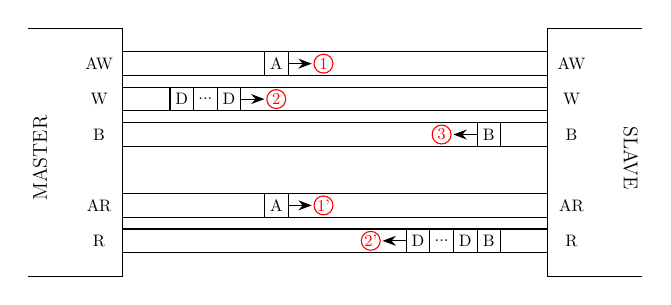
\begin{tikzpicture}[scale=0.6, every node/.style={scale=0.6}]
    % Module Master
    \draw ( 0.0, 0.0) -- ++( 2.0, 0.0) -- ++( 0.0, 5.25) -- ++( -2.0, 0.0);
    \node[rotate=90] at (0.25, 2.5) {\large MASTER};
    % Module Slave
    \draw (13.0, 0.0) -- ++(-2.0, 0.0) -- ++( 0.0, 5.25) -- ++( 2.0, 0.0);
    \node[rotate=270] at (12.75, 2.5) {\large SLAVE};
    % AW channel
    \node at ( 1.5, 4.50) {AW};
    \draw ( 2.0, 4.25) rectangle ++( 9.0, 0.5);
    \draw ( 5.0, 4.25) rectangle ++( 0.5, 0.5)  node[pos=.5] {A};
    \draw[-{Stealth}] ( 5.5, 4.5) -- ++( 0.5, 0.0);
    \node at ( 11.5, 4.50) {AW};
    \draw[red] ( 6.25, 4.50) circle [radius=0.2] node {1};
    % W channel
    \node at ( 1.5, 3.75) {W};
    \draw ( 2.0, 3.50) rectangle ++( 9.0, 0.5);
    \draw ( 3.0, 3.50) rectangle ++( 0.5, 0.5)  node[pos=.5] {D};
    \draw ( 3.5, 3.50) rectangle ++( 0.5, 0.5)  node[pos=.5] {...};
    \draw ( 4.0, 3.50) rectangle ++( 0.5, 0.5)  node[pos=.5] {D};
    \draw[-{Stealth}] ( 4.5, 3.75) -- ++( 0.5, 0.0);
    \node at ( 11.5, 3.75) {W};
    \draw[red] ( 5.25, 3.75) circle [radius=0.2] node {2};
    % B channel
    \node at ( 1.5, 3.00) {B};
    \draw ( 2.0, 2.75) rectangle ++( 9.0, 0.5);
    \draw ( 9.5, 2.75) rectangle ++( 0.5, 0.5)  node[pos=.5] {B};
    \draw[-{Stealth}] ( 9.5, 3.00) -- ++(-0.5, 0.0);
    \node at ( 11.5, 3.00) {B};
    \draw[red] ( 8.75, 3.00) circle [radius=0.2] node {3};
    % AR channel
    \node at ( 1.5, 1.50) {AR};
    \draw ( 2.0, 1.25) rectangle ++( 9.0, 0.5);
    \draw ( 5.0, 1.25) rectangle ++( 0.5, 0.5)  node[pos=.5] {A};
    \draw[-{Stealth}] ( 5.5, 1.5) -- ++( 0.5, 0.0);
    \node at ( 11.5, 1.50) {AR};
    \draw[red] ( 6.25, 1.50) circle [radius=0.2] node {1'};
    % R channel
    \node at ( 1.5, 0.75) {R};
    \draw ( 2.0, 0.50) rectangle ++( 9.0, 0.5);
    \draw ( 8.0, 0.50) rectangle ++( 0.5, 0.5)  node[pos=.5] {D};
    \draw ( 8.5, 0.50) rectangle ++( 0.5, 0.5)  node[pos=.5] {...};
    \draw ( 9.0, 0.50) rectangle ++( 0.5, 0.5)  node[pos=.5] {D};
    \draw ( 9.5, 0.50) rectangle ++( 0.5, 0.5)  node[pos=.5] {B};
    \draw[-{Stealth}] ( 8.0, 0.75) -- ++(-0.5, 0.0);
    \node at ( 11.5, 0.75) {R};
    \draw[red] ( 7.25, 0.75) circle [radius=0.2] node {2'};
\end{tikzpicture}

        \caption{Caption}
        \label{fig:axi_transaction_scheme_figure}
    \end{figure}

\section{Design Goals and Overview}\label{sec:overview}

\begin{figure*}
  \centering
  \includegraphics[width=1\textwidth]{images/SchIM_diagram.png}
  \caption{Internal logic organization of the \schim connected to the
    PS through the HPM, LPM and HPS ports.}
  \label{fig:MemorEDF_module_schema}
\end{figure*}

%% General introduction about the SchIM
In this section, we introduce the proposed \schim design and describe
the overarching goals of this work. We then provide a bird's-eye view
of the \schim organization and principles of operation.

\subsection{Design Goals}\label{sec:design_goals}
As briefly surveyed in Section~\ref{sec:relwork}, there have been
numerous proposals for better memory controllers and approaches to
manage memory traffic in modern multi-core embedded platforms. With
respect to the existing literature, the purpose of this work is
twofold. First, we want to demonstrate that scheduling CPU-originated
memory traffic at the granularity of individual transactions is
possible in PS-PL platforms. Second, and more importantly, we want to
provide an infrastructure that is generic and extensible enough for
the broader research community to adopt and foster a new chapter on
PL-assisted memory scheduling. With this in mind, we establish the
following goals.

\par{\bf Extensible memory scheduling infrastructure.} First and
foremost, the \schim has been designed with modularity and
extensibility in mind. We separate the functionalities that concern
handling, queuing, selection, and forwarding of memory requests inside
our infrastructure. Moreover, we design our \schim to be able to support multiple memory scheduling policies simultaneously. A simple,
standardized interface is provided to define new memory scheduling
policies without impacting the design of the rest of the \schim. We
discuss in Section~\ref{sec:sched_interf} the generic interface
provided by the \schim to implement a new memory scheduling policy.

\par{\bf Runtime configuration and transparency.} We want the \schim
to be a robust supporting infrastructure to evaluate, compare, and
contrast memory scheduling policies. As such, we strive to provide (1)
runtime reconfigurability and (2) operational transparency. It is possible to rapidly identify desirable configuration parameters by
allowing memory scheduling policies to be switched at runtime. Besides, an adopted policy can be tuned according to the workload criticality and memory intensiveness. For this purpose, the \schim exposes a memory-mapped
configuration interface where all the operational parameters can be
changed at runtime. At the same time, we want to ensure that the
applications and the (real-time) operating system under analysis need
not be modified to use the \schim. Hence, we propose using a
thin virtualization layer to selectively route memory traffic through
the \schim without changes to the binary of OS kernel and
applications.

\par{\bf Realistic performance with experimental policies.} One of the
limiting factors of research on memory scheduling policies is the
ability to construct evidence of performance improvements with
the realistic workload. Proposing a new memory scheduling policy is
traditionally done with either a simulated setup or with a
full-system soft-core implementation. Both cases are considerably slower than what it would be in real systems and force the use of an unrealistically lightweight workload. Nonrealistic workloads limit the repeatability of experiments of scale.

Furthermore, the multi-fold drop in performance excludes the
possibility of adopting experimental memory scheduling policies for a
production-ready system. Conversely, we envision that our \schim will
be an intermediate step in the transition path to the production of
research-seeded ideas. Additionally, as PS-PL platforms mature and the interplay of PL and memory resources improves, a \schim-like design
could be the way to go for mission-reconfigurable, upgradable embedded
systems.

\subsection{Design Overview}
As previously mentioned, the \schim leverages the PLIM
approach. CPU-originated main memory transactions are re-routed
through the programmable logic and scheduled by the \schim according
to a flexible and configurable policy. The result is that the timing
of memory transactions generated by real-time applications can be
carefully determined and reasoned upon. Because the \schim follows a
PLIM approach, transactions can be selectively sent to the \schim for
scheduling. However, it is always possible to dynamically exclude the
\schim and route transactions directly to the main memory. Toward this paper's incentive, we consider a setup in which \schim handles all the CPU-generated memory transactions.

%% First and foremost, SchIM follows a selective and dynamic re-routing
%% policy settled at the runtime, meaning that provided a proper routing
%% configuration interface, SchIM can be bypassed if unacceptable
%% overhead for some applications is detected by going through the PL
%% following the Loop-Back routing strategy. Additionally, SchIM,
%% provides a safe production-ready environment on COTS platforms where
%% one can enfroce and test any proposed scheduling policy at the level
%% of the transaction altogether by the real hardware. Memory scheduling
%% traditionally done via hardware modifications at the controller level,
%% or solely via software. Providing SchIM, we are now able to transcend
%% this on intact COTS to conduct an analysis of feasibility, challenges
%% and performance.

\fig{fig:PS-PL-diagram} provides an overview of the location of the
\schim in the reference platform, while its internal organization is
visible in \fig{fig:MemorEDF_module_schema}. Application memory
requests reach the \schim the aforementioned HPM ports. Without loss
of generality, we consider a \schim instance with two arrival lanes,
which are labeled as \axiin{1} and \axiin{2} in
\fig{fig:MemorEDF_module_schema}. The \schim then forwards the
received transactions towards main memory through the \axiout{}
interface. A more detailed view of the \schim module is provided in
\fig{fig:MemorEDF_module_schema} where the same convention is used to
identify input and output ports. In addition, as shown in
\fig{fig:MemorEDF_module_schema}, a fourth \axiconf{} port is used to
configure the \schim from the PS.

%% The objective of the module is to arbitrate the access of the bus to
%% the main memory between the different cores of the PS side at the
%% transaction level by enforcing a given policy.  Roughly, the module
%% receives transactions from the PS side, acknowledges them and finally
%% repeat them with the main memory as destination.  The exact order in
%% which inter-core transactions are being repeated is decided by an
%% embedded on-chip hardware scheduler.

%% \begin{figure}
%%   \centering
%%   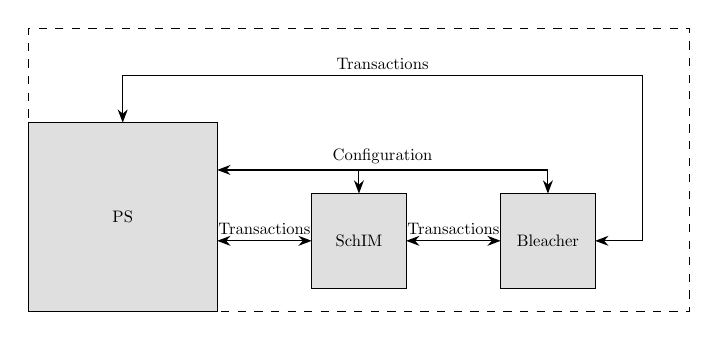
\begin{tikzpicture}[scale=0.6, every node/.style={scale=0.6}]
    % Modules
    \draw[fill={rgb:black,1;white,7}] ( 0.0, 0.0) rectangle ( 4.0, 4.0) node[pos=.5] {PS};
    \draw[fill={rgb:black,1;white,7}] ( 6.0, 0.5) rectangle ( 8.0, 2.5) node[pos=.5] {SchIM};
    \draw[fill={rgb:black,1;white,7}] (10.0, 0.5) rectangle (12.0, 2.5) node[pos=.5] {Bleacher};
    % Outline PL
    \draw[dashed] ( 0.0, 4.0) -- ( 4.0, 4.0) -- ( 4.0, 0.0) -- (14.0, 0.0) -- (14.0, 6.0) -- ( 0.0, 6.0) -- ( 0.0, 4.0);
    % Buses
    % PS to SchIM HPM0
    \draw[{Stealth}-{Stealth}] ( 4.0, 1.5) -- ( 6.0, 1.5) node[above, pos=.5] {Transactions};
    % SchIM to Bleacher HPM0
    \draw[{Stealth}-{Stealth}] ( 8.0, 1.5) -- (10.0, 1.5) node[above, pos=.5] {Transactions};
    % SchIM to Bleacher HPM0
    \draw[{Stealth}-{Stealth}] (12.0, 1.5) -- (13.0, 1.5) -- (13.0, 5.0) -- ( 2.0, 5.0) node[above, pos=.5] {Transactions} -- ( 2.0, 4.0);
    % PS to SchIM and Bleacher LPD
    \draw[{Stealth}-{Stealth}] ( 4.0, 3.0) -- (11.0, 3.0) node[above, pos=.5] {Configuration} -- (11.0, 2.5);
    \draw[-{Stealth}] ( 7.0, 3.0) -- ( 7.0, 2.5);
\end{tikzpicture}

%%   \caption{High-level block design of the proposed \schim
%%     module. \emph{RM: we need to replace this picture with one that
%%       provides more details about the main blocks of the platforms. We
%%       also do not need to include the bleacher as it is not
%%       fundamental for the operation of the \schim.}}
%%   \label{fig:SchIM_overview_schema}
%% \end{figure}


%% Micro-architecture and first list of modules
The \schim module is composed of a number of sub-modules grouped into
three different domains, namely (i) the \emph{interfacing domain},
(ii) the \emph{queuing domain}, and (iii) the \emph{scheduling
  domain}.

\par{\bf The interfacing domain} encompasses the sub-modules to
interface the core logic of the \schim with the rest of the system
using the AXI protocol.  This is comprised of three sub-modules. These
are (i) the \emph{packetizer(s)}, (ii) the \emph{serializer}, and
(iii) the previously mentioned \emph{configuration} interface.

The PS-facing end of the {\bf packetizer} offers an AXI slave port to
accept new incoming transactions. Upon receipt, this module transforms
each transaction into an equivalent \emph{packet} that can be queued
and scheduled by \schim. Packetization of AXI
transactions is necessary to be able to store transactions that are
serial by nature.  A standard AXI transaction is composed of
one address phase (AR or AW channel) followed by a data phase (R or W
channel), which can be itself composed of multiple successive bursts.

In many ways, the {\bf serializer} is the dual module of the
packetizer. Its purpose is to transform the packets that encode
CPU-generated memory requests back into AXI-compliant transactions. As
such, the serializer offers a master port to the rest of the system to
be routed to the main memory controller.

%% purpose of slave and master ports, they are also in charge of
%% respectively transforming the AXI transactions into an equivalent
%% packet and to transform these packets

\par{\bf The queuing domain} handles how packets are stored between
receipt and re-trasnmission. This domain is comprised of (i) the
\emph{dispatcher} module, (ii) the \emph{transaction queues}, and
(iii) the \emph{selector} module.

The use of {\bf multiple transaction queues} is necessary to
differentiate the traffic of the CPUs and perform scheduling. As such,
the \schim associates a queue to each of the active cores --- four in
the platform of reference.
%% Therefore, in order to cancel the Round Robin arbitration policy
%% applied in the PS side and in order to avoid that one high priority
%% core is stalled by a lower priority one, each core is granted a queue
%% within the \schim module. <-- This should be obvious (RM)
The queues implemented in the \schim not only act as a holding space
for in-flight memory transactions.  They also (a) provide information
to the scheduling domain regarding their current state, and (b) they
can generate a congestion control signal to the associated CPU
core.

Congestion control is vital because memory transactions originated
at the LLC controller follow the same route to the \schim regardless
of the originating CPU. Typically, the total number of outstanding
transactions that the cores can emit exceeds the queuing elements' capacity on the loop-back route. Hence, priority inversion arises if a low-priority CPU's memory traffic is (temporarily) held. Latter is due to the uncontrolled queue buildup, which provokes a head-of-line blockage. Importantly, what described is true also for the normal
route and it is a direct consequence of the best-effort nature of
traditional multi-core memory buses. The \schim allows the user to
specify a configurable threshold on the occupancy of the queues that,
when reached, issues a regulation signal to the corresponding CPU. We
describe in greater detail how congestion control was implemented on
the target platform in Section~\ref{sec:pl-to-ps-feedback}.

As suggested by \fig{fig:MemorEDF_module_schema}, transactions are
categorized and enqueued based on the source of traffic. The {\bf
  dispatcher} module performs the matching between an incoming
transaction and the destination queue. Similarly, transactions are
dequeued by the {\bf selector} module and sent directly to the output
of the \schim following the scheduling domain's resolutions.

\par{\bf The scheduling domain} encompasses all the sub-modules that
enable arbitration of transactions issued by the different cores of
the PS. The modules in this domain are intended to be generic for
extensibility, albeit the first set of three template schedulers is
provided as a proof of concept.  The scheduling policies currently
implemented in the \schim are Fixed Priority (FP), Time Division
Multiple Access (TDMA), and Budget-based Traffic Shaping (TS).  Each
of the parameters required by the implemented policies --- such as the
priorities, the periods, and the budgets --- can be adjusted at
runtime via the configuration interface.

The FP scheduler allows associating a priority value to each of the
transaction queues. Pending transactions at the queues are then
forwarded out of the \schim following the user-defined priority
order. The TDMA scheduler allows associating a transmission time slot
to each of the queues expressed in PL clock cycles. The module then
builds a schedule by concatenating the per-core slots so that only
pending transactions from one queue at a time are forwarded by the
\schim. Finally, with the TS scheduler, it is possible to associate a
maximum rate at which transactions from each queue are forwarded by
the \schim.

%% Finally, the scheduling domain is also the one in charge of the
%% control of the remaining \schim module, driving and selecting the
%% adequate signals and ensuring the coherence and integrity of the data.

%% \subsection{Modules Overview}

%% \par{\bf Packetizer:} The packetizer module transforms transactions on
%% the asynchronous AXI bus into schedulable entities to be queued at any
%% of the \schim queues.

%\section{Theoretical Background}
    \subsection{Fixed Priority}
    \subsection{Time Division Memory Access}
    \subsection{Earliest Deadline First}
    \subsection{Least Laxity First}
    \subsection{MemGuard}
\section{SchIM Implementation}
    As previously mentioned, SchIM is a PLIM module that performs a memory loop-back through the PL side similarly to \cite{PLIM20}.
    The objective of the module is to arbitrate the access of the bus to the main memory between the different cores of the PL side at the transaction level by enforcing a given policy.
    Roughly, the module receives transactions from the PS side, acknowledges them and finally repeat them with the main memory as destination.
    The exact order in which inter-core transactions are being repeated is decided by an embedded on-chip hardware scheduler.

    \subsection{Communication scheme}
        The exact communication scheme varies depending on whether the transaction aims at reading the main memory or writing to it as emphasised in the figures \ref{fig:Write_SchIM_communication_scheme} and \ref{fig:Read_SchIM_communication_scheme}.
        This difference between the schemes is a direct consequence of the AXI protocol used.
        As illustrated in the figure \ref{fig:Write_SchIM_communication_scheme}, the writing scheme is a simple succession of two standard AXI transactions. In fact, the actions groups $1-2-3$ and $4-5-6$ are both the succession of an address phase, followed by a data phase itself followed by a response phase.

        On the other hand, the reading communication scheme is a less linear as the cores are not unloading some data but rather retrieve some.
        The main difference with the writing scheme lays in the fact that the entire transaction is only partially pipelined.
        As depicted in the figure \ref{fig:Read_SchIM_communication_scheme}, steps 1 and 2 can be pipelined however, the PS is still busy waiting for the data to arrive whereas, in figure \ref{fig:Write_SchIM_communication_scheme}, once the step 3 is completed, the core can resume.

        \begin{figure}
            \begin{subfigure}{.5\textwidth}
                \centering
                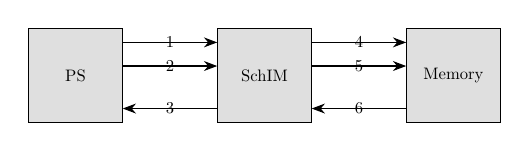
\begin{tikzpicture}[scale=0.6, every node/.style={scale=0.6}]
    % States
    \draw[fill={rgb:black,1;white,7}] ( 0.0, 0.0) rectangle ( 2.0, 2.0) node[pos=.5] {PS};
    \draw[fill={rgb:black,1;white,7}] ( 4.0, 0.0) rectangle ( 6.0, 2.0) node[pos=.5] {SchIM};
    \draw[fill={rgb:black,1;white,7}] ( 8.0, 0.0) rectangle (10.0, 2.0) node[pos=.5] {Memory};
    % Edges
    % PS to SchIM Address phase
    \draw[-{Stealth}] (2.00, 1.70) -- (4.00, 1.70) node[pos=.5] {1};
    % PS to SchIM Data phase
    \draw[-{Stealth}] (2.00, 1.20) -- (4.00, 1.20) node[pos=.5] {2};
    % PS to SchIM
    \draw[{Stealth}-] (2.00, 0.30) -- (4.00, 0.30) node[pos=.5] {3};
    % SchIM to Memory Address phase
    \draw[-{Stealth}] (6.00, 1.70) -- (8.00, 1.70) node[pos=.5] {4};
    % SchIM to Memory Data phase
    \draw[-{Stealth}] (6.00, 1.20) -- (8.00, 1.20) node[pos=.5] {5};
    % SchIM to Memory
    \draw[{Stealth}-] (6.00, 0.30) -- (8.00, 0.30) node[pos=.5] {6};
\end{tikzpicture}

                \caption{The six phases required to perform a write transaction}
                \label{fig:Write_SchIM_communication_scheme}
            \end{subfigure}
            \par\bigskip
            \begin{subfigure}{.5\textwidth}
                \centering
                \input{tikz/read_SchIM_communication_scheme}
                \caption{The four phases required to perform a read transaction}
                \label{fig:Read_SchIM_communication_scheme}
            \end{subfigure}
            \caption{Sequence of phases in order to perform a read (a) or write (b) memory transaction from the PS to the memory by going through SchIM.}
            \label{fig:SchIM_communication_scheme}
        \end{figure}

    \subsection{Micro-architecture}
        The SchIM module is composed of many submodules that can themselves be grouped into three different domains. In fact, as illustrated in figure \ref{fig:MemorEDF_module_schema}, one can distinguish the \emph{scheduling domain}, the \emph{queueing domain} and the \emph{interfacing domain}.

        The scheduling domain encompasses all the sub-modules that enable arbitration of the bus the transactions issued by the different cores of the PS side. Hence, this domain boasts several transaction schedulers implemented at the hardware level.
        The scheduling policies offered by SchIM include Fixed Priority (FP), Time Division Multiple Access (TDMA), Earliest Deadline First (EDF), Least Laxity First (LLF) and MemGuard (MG).
        Each of the parameters required by the aforementioned algorithms such as the priorities, the periods, the deadlines and the budgets are re-configurable at the run-time thanks to the inclusion of a configuration port.
        Finally, the scheduling domain is also the one in charge of the control of the remaining the SchIM module, driving and selecting the adequate signals to the adequate sub-modules with the appropriate timing.

        The queueing domain is in charge of the storing the incoming transactions emitted by the PS side.
        The motivation behind th euse of queues is implied by the fact that all the masters located on the PS side must share a common AXI bus (namely HPM0 as shown in figure \ref{fig:SchIM_overview_schema}).
        Therefore, in order to cancel the Round Robin arbitration policy applied in the PS side and in order to avoid that one high priority core is stalled by a lower priority one, each core is granted a queue within the SchIM module.
        Not only the queues act as containers for transactions, they also embed logic and provide information to the scheduling domain regarding their current state in order to avoid the queues to overflow or underflow similarly to the producer-consumer problem.
        As suggested by figure \ref{fig:MemorEDF_module_schema}, transactions are inserted to the adequate queues on the basis of the emitters identifier via the dispatcher module.
        Similarly, transactions are evicted from their queue, routed by the selector module and sent directly to the output of the module upon the action of the scheduling domain.

        The interfacing domain encompases the submodules in charge of interfacing both the scheduling domain and the queuing domain with the remaining of the system using the AXI protocol.
        More accurately, three modules compose this domain, the configuration port previously mentioned, the packetizer and the serializer.
        While the packetizer and the serializer serve the purpose of slave and master ports, they are also in charge of respectively transforming the AXI transactions into an equivalent packet and to transform these packets back to a AXI compliant transactions.
        The need for packetizing (i.e. flattening) the AXI transactions is driven by the necessity of storing transactions that are inherently serial (for AXI, one address phase followed by a data phase itself composed of multiple successive bursts) within the queuing domain.

        \begin{figure}
            \centering
            \includegraphics[scale=0.08]{images/MemorEDF_module_schema.png}
            \caption{Caption}
            \label{fig:MemorEDF_module_schema}
        \end{figure}

    \subsection{Transactions Life Cycle}
    Let us consider a system with four cores (noted $C = \{c_{0}, c_{1}, c_{2}, c_{3}\}$) sending transactions $T = \{t_{0}, t_{1}, ..., t_{n}\}$ to the SchIM module.
    Consequently, the latter boasts four queues (noted $Q = \{q_{0}, q_{1}, q_{2}, q_{3}\}$) buffering the transactions under the form of packets $P = \{p_{0}, p_{1}, ..., p_{n}\}$ where $p_{i} = Packetizer(t_{i})~\forall i \in [0 : n]$.

    In the present example, we will assume $t_{1}$ as being the transaction under analysis.
    The latter is emitted by $c_{2}$ in direction of the SchIM module.
    The packetizer receives this transaction and, once the AXI protocol completed, transform it into an equivalent packet $p_{1} = Packetizer(t_{1})$.
    Following this transformation, the newly created packet is forwarded to the dispatcher which, thanks to the emitter's id embedded within the transaction, is re-routed to the corresponding queue $q_{2}$ (since emitted by $c_{2}$).
    After the insertion of $p_{1}$ in $q_{2}$, the state of the queuing domain is as follows: $q_{0}$ has two packets $p_{0}$ and $p_{k}$ and $q_{2}$ only has $p_{1}$.
    At this point, $q_{0}$ is considered for scheduling by the scheduling domain.
    In consequence, $p_{0}$ is forwarded to the serializer through the selector.
    Simultaneously to the reception of the packet by the serializer, the latter receives an activation signal from the scheduling domain informing the serializer that the packet is valid and that a transaction can be started.
    Similarly to the packetizer, the serializer will transform the packet $p_{0}$ back to its initial AXI transaction form $t_{0} = Serializer(p_{0})$.
    Thereafter, once the $t_{0}$ has been sent, the serializer will inform the scheduling domain via a signal, that he is ready to accept the next packet as input.
    Upon the reception of this signal, the scheduling domain will both re-direct the latter to the queue of the previous packet to indicate that it has been consumed and change the selected queue according to the scheduling policy so that the first packet of this queue can be forwarded to the serializer thought the selector module.
    In the present example, the "consumed" signal forwarded by the scheduler is sent to $q_{0}$ which is then empty.
    At this point, two scenarios are still possible.
    \begin{enumerate}
        \item $q_{0}$ is still considered for scheduling following the selected scheduling policy. Therefore, as $q_{0}$ is empty, it outputs an "empty" signal received by the scheduler.
              The latter then decides to not send any activation signal because there is nothing to left to read in the selected queue.
              In other words, the access to the main is stalled on purpose by the scheduling policy i.e. the scheduling policy is not work conserving.
              For instance, such a scenario could happen in the case of TDMA or if all the queues are empty.
              The logic will resume as soon as the selected queue is filled.
        \item $q_{2}$ is now considered instead of $q_{0}$.
              In this case, the "consumed" signal is sent to $q_{0}$ while the queue ID changes in order to select $q_{2}$.
              This results in the packet contained inside $q_{1}$ to be forwarded to the selector.
    \end{enumerate}

\subsection{PL-to-PS Feedback}
\label{sec:pl-to-ps-feedback}
Each of the HPM ports interfacing the PS and the PL sides (HPM1 and
HPM2) have two dedicated queues for read and write transactions. Since
transactions are being buffered inside \schim as well as in these port
buffers, head-of-line blocking can happen. Head-of-the-line blocking
is harmful for performance; and can cancel out the benefits of
transaction scheduling performed by the \schim. For instance, in the
case of a non work-conserving policy (e.g., TDMA), if the HPM port
queue gets filled with transaction coming for the same core, no other
transaction will be able to reach the \schim and thus be considered
for scheduling. This implies that no transaction would be scheduled
until the end of the active core's TDMA slot. On the other hand, for
work-conserving policies (e.g., FP) in the presence of head-of-line
blocking, the decisions being taken by \schim would directly depend on
the order at which transactions are emitted by the HPM port buffer.

In both cases, one must prevent the cores from saturating the HPM port
buffers. In order to avoid such situation, we implemented a feedback
scheme aimed at slowing down the cores when necessary. As we mentioned
in the context of \fig{fig:MemorEDF_module_schema}, the \schim's
queues are associated a programmable threshold. Whenever the queue
occupancy reaches (or exceeds) the associated threshold, a per-core
interrupt line is asserted from the PL to the PS side. When received,
the interrupt is treated by the platform software as a \emph{fast
  interrupt request} (FIQ) and directly handled by the
hypervisor---invisible to any guest OS. The advantage of using FIQs
instead of regular IRQs is the significantly reduced handling
latency~\cite{fiq_results}. Minor modifications to the TrustZone
monitor were necessary to correctly configure FIQ handling. To
minimize overhead, the installed FIQ handler only executes two
assembly instructions. These are (1) a \texttt{dsb} memory barrier
that stops the core until all the outstanding memory transactions have
been completed, and (2) a \texttt{eret} instruction to exit the FIQ
context. There is not need to save/restore any register because FIQs
have banked syndrome/status registers and because no general purpose
register is modified in the handler.

Ideally, the available space in the HPM buffers should be shared
evenly between the cores. Since each HPM port has a buffer with a
depth of 8+8 transactions, each core should occupy at most 2 slots in
each buffer. Unfortunately, our experiments highlighted that the
control over amount of transactions buffered by each core is
imperfect. Often times, the selected threshold is exceeded by up to
two transactions. This is the main reason why we propose a dual-ported
\schim which uses both the available HPM ports. Indeed, by assigning
two cores on each of the ports, the ideal threshold on maximum amount
buffered transactions can be doubled. The increase provides enough
room to compensate for imperfections in the micro-regulation performed
with PL-to-PS FIQ delivery.

\begin{comment}
    \subsection{Transactions Life Cycle}
\label{subsec:transaction-life-cycle}

Let us consider a system with four cores $c_0, \ldots, c_3$ sending
transactions $T = \{t_{0}, t_{1}, ..., t_{n}\}$ to the \schim module.
Consequently, the latter boasts four queues (noted $Q = \{q_{0},
q_{1}, q_{2}, q_{3}\}$) buffering the transactions under the form of
packets $P = \{p_{0}, p_{1}, ..., p_{n}\}$ where $p_{i} =
Packetizer(t_{i})~\forall i \in [0 : n]$.

In the present example, we will assume $t_{1}$ as being the
transaction under analysis.  The latter is emitted by $c_{2}$ in
direction of the \schim module.  The packetizer receives this
transaction and, once the AXI protocol completed, transform it into an
equivalent packet $p_{1} = Packetizer(t_{1})$.  Following this
transformation, the newly created packet is forwarded to the
dispatcher which, thanks to the emitter's id embedded within the
transaction, is re-routed to the corresponding queue $q_{2}$ (since
emitted by $c_{2}$).  After the insertion of $p_{1}$ in $q_{2}$, the
state of the queuing domain is as follows: $q_{0}$ has two packets
$p_{0}$ and $p_{k}$ and $q_{2}$ only has $p_{1}$.  At this point,
$q_{0}$ is considered for scheduling by the scheduling domain.  In
consequence, $p_{0}$ is forwarded to the serializer through the
selector.  Simultaneously to the reception of the packet by the
serializer, the latter receives an activation signal from the
scheduling domain informing the serializer that the packet is valid
and that a transaction can be started.  Similarly to the packetizer,
the serializer will transform the packet $p_{0}$ back to its initial
AXI transaction form $t_{0} = Serializer(p_{0})$.  Thereafter, once
the $t_{0}$ has been sent, the serializer will inform the scheduling
domain via a signal, that he is ready to accept the next packet as
input.  Upon the reception of this signal, the scheduling domain will
both re-direct the latter to the queue of the previous packet to
indicate that it has been consumed and change the selected queue
according to the scheduling policy so that the first packet of this
queue can be forwarded to the serializer through the selector module.
In the present example, the "consumed" signal forwarded by the
scheduler is sent to $q_{0}$ which is then empty.  At this instant,
two scenarios are possible:

\begin{enumerate}
\item $q_{0}$ is still considered for scheduling following the
  selected scheduling policy. Therefore, as $q_{0}$ is empty, it
  outputs an "empty" signal received by the scheduling domain.  The
  latter then decides to not send any activation signal to the
  serializer because there is nothing left to transmit in the selected
  queue.  In other words, the access to the main memory is being
  stalled on purpose by the scheduling policy i.e. the scheduling
  policy is not work conserving.  For instance, such a scenario could
  happen in the case of TDMA or if all the queues are empty.  The
  logic will resume as soon as the selected queue is filled.
\item $q_{2}$ is now considered instead of $q_{0}$ for scheduling.  In
  this case, the "consumed" signal is repeated to $q_{0}$ while the
  queue ID changes in order to select $q_{2}$.  This results in the
  packet contained inside $q_{1}$ to be forwarded to the selector.
\end{enumerate}
\end{comment}

\section{Evaluation}

We have performed a full system implementation on a Xilinx ZCU102 development board, featuring a Xilinx Zynq UlraScale+ XCZU9EG SoC. For this work, we utilize a combination of synthetic and real benchmarks. Our synthetic benchmark.
\todo[inline]{
  Talk about IO intensive and memory intensive benchmarks to be designed....
  We also include a study of the behavior of real applications from the San Diego Vision Benchmark Suite (SD-VBS) \cite{SD-VBS}, which comes with multiple input sizes....
}
\todo[inline]{
    DH: Maybe we could use AES from MiBench ?
}

As mentioned earlier, the high-performance master ports, namely HPMs, serve as a gateway from the PS to the PL. We implemented our scheduler IP, SchIM, responding under the physical addresses of HPM0 right after the PS. By doing so, any transaction toward the PL has to go through the SchIM. Hence, all memory requests yield to the scheduling policy being enforced by the scheduler. Design features of SchIM implementation and configuration interface are detailed in section ??.


At the preprocessing stages, an AXI Performance Monitor (APM) unit connected to the bus interface between the HPM0 and the scheduler. It is crucial to affirm that this medium does not affect the transaction flow toward the PL.  APMs are powerful tools available in the PS and instantiable in the PL capable of measuring primary performance metrics (for AXI4, AXI4-Lite, or AXI4-Stream-based systems) such as bus latency for specific master/slave or amount of memory traffic for the particular duration. Moreover, APM offers the functionality of logging the necessary information about data transfers between any master and slave communicating in the AXI protocol. In this work, we program APMs to profile the behavior of the benchmarks to analyze the task's deadline. SchIM employs profiled information on task deadlines to make scheduling decisions (e.g., enforce EDF policy) for hard real-time jobs.

  \subsection{Performance degradation}

  \subsection{Platform Capabilities}
    Here, discuss Fig.\ref{fig:bandwidth_comparison}
    \todo[inline]{Broad evaluation of the bandwidth offer by the ZCU102 depending on the route considered.}
    \begin{figure}
      \centering
      \includegraphics[scale=0.5]{../doc/experiments/bw_comparisons.png}
      \caption{Board bandwidth}
      \label{fig:bandwidth_comparison}
      \todo[inline]{TODO: outdated version. Has to be repeated for cached transactions only with the latest version of SchIM.}
    \end{figure}

  \subsection{Internal Behaviour of SchIM}
    Here, show and emphasize on the behaviour of SchIM with Fig.\ref{fig:schim_behaviour}
    \todo[inline]{Here, we use the trace snapshots}
    \begin{figure*}
      \begin{subfigure}{.31\textwidth}
        \centering
        % include first image
        \includegraphics[scale=0.31]{images/iladata_fp_3_0f0e0d0c_20_3.png}
        \caption{FP with ordering $C_{3} \succ C_{2} \succ C_{1} \succ C_{0}$}
        \label{fig:schim_behaviour_fp}
      \end{subfigure}
      \hfill
      \begin{subfigure}{.31\textwidth}
        \centering
        % include second image
        \includegraphics[scale=0.31]{images/iladata_tdma_3_3_512_512_1.png}
        \caption{TDMA with slots of 512 clock cycles}
        \label{fig:schim_behaviour_tdma}
      \end{subfigure}
      \hfill
      \begin{subfigure}{.31\textwidth}
        \centering
        % include second image
        \includegraphics[scale=0.31]{images/iladata_mg_3_128_128_3.png}
        \caption{MG with min. period of 128 clock cycles}
        \label{fig:schim_behaviour_mg}
      \end{subfigure}
      \caption{Trace snapshot of SchIM for the three implemented policies}
      \label{fig:schim_behaviour}
      \todo[inline]{TODO: The plots have to be reworked.}
    \end{figure*}

  \subsection{Memory Isolation}
%    \todo[inline]{Here, prove that SchIM enables us to isolate the cores. We need a bunch of benchmarks competing with mem-bombs on the remaining cores. We will try:
    \begin{itemize}
      \item FP:~ The benchmark running alone with the highest priority VS. the same setup with mem-bombs
      \item TDMA:~ The benchmark running alone with all the cores having a slot of the same size VS. the same setup with mem-bombs
      \item MG:~ The benchmark running alone with all the cores having a given periodicity VS. the same setup with mem-bombs
    \end{itemize}
%    }

\section{Discussion}
    When comparing the throughput that is experienced by the cores, the normal route always provides a higher throughput in comparison to the the loop-back based path.
    However, when only comparing those loop-back based paths, we can see that the price to pay for having \schim is largely compensated by the memory isolation the latter enables.
    In general, using redirecting the cores traffic toward the PL side with \schim is interesting in combination with techniques such \textit{address bleaching} and \textit{zero-copy recoloring}.

\section{Conclusion}
    \begin{itemize}
        \item The authors acknowledge that the described phenomenon is unlikely to happen in a mainstream platform, or if it happens, the consequences are negligeable. Nonethless, this experiment has the merit of pinpointing a malfunction in the last level of cache controller of the ARM Cortex-A53. The experiment also shed light on the importance of selecting trustable 3thr party IPs and designing correctly IPs if they are cacheable target memories.
        \item Such system, under strict conditions cannot quarantee QoS nor Mixed-criticality levels.
        \item In contrast to what has been previously reported, read intensive applications can also become a threat for the system predictability.
        \item Bus slaves must be designed carefully to provide fast answers. More specifically, SoCs featuring a tightly integrated FPGA must ensure that the FPGA can only be reprogrammed by a trusted actor as simply holding a single transaction can indefinitely stall the whole core cluster.
    \end{itemize}

    \subsection{Future works}
        \begin{itemize}
            \item Study if the same impact can be found with the attacker targeting a scratch pad memory which frequency could be modify.
        \end{itemize}


\bibliographystyle{IEEEtranS}
\bibliography{references}

\end{document}
